\documentclass[conference]{IEEEtran}
\IEEEoverridecommandlockouts
% The preceding line is only needed to identify funding in the first footnote. If that is unneeded, please comment it out.
\usepackage{cite}
\usepackage{amsmath,amssymb,amsfonts}
\usepackage{algorithmic}
\usepackage{graphicx}
\usepackage{textcomp}
\usepackage{xcolor}
\def\BibTeX{{\rm B\kern-.05em{\sc i\kern-.025em b}\kern-.08em
    T\kern-.1667em\lower.7ex\hbox{E}\kern-.125emX}}
\begin{document}

\title{RFID Sicherheit}


\author{\IEEEauthorblockN{Julian Hoever}
\IEEEauthorblockA{\textit{Verteilte Systeme} \\
\textit{Universität Duisburg-Essen}\\
Duisburg, Deutschland\\
julian.hoever@stud.uni-due.de}
}

\maketitle

\begin{abstract}
Die folgende Arbeit behandelt das Thema der RFID Sicherheit im Bezug auf Sicherheitslücken, Schutzmaßnahmen und Privatsphäre. Es werden einige mögliche Schwachstellen der RFID/NFC Technik aufgezeigt und Angriffstechniken vorgestellt, welche die zuvor aufgeführten Schwachstellen ausnutzen. Dabei wird darauf eingegangen, in welchen realen Szenarien diese Angriffe eine Bedrohung darstellen (kontaktloses Bezahlen, Diebstahlsicherung von Waren). Anschließend werden einige Schutzmaßnahmen skizziert, welche die zuvor genannten Angriffstechniken abmildern oder verhindern können und es wird diskutiert, wie durchführbar die genannten Angriffstechniken in der realen Welt sind. Dies hilft dabei abzuschätzen, wie relevant die Bedrohung ist, die von der RFID Technik in diesen Bereichen ausgeht. Abschließend wird noch der Aspekt der Einschränkung der Privatsphäre durch RFID Chips, besonders in Ausweisen aber auch in Produkten zur Diebstahlsicherung, besprochen und eingeordnet.
\end{abstract}

\section{Einleitung}
Die kontaktlose RFID Technik gehört bei vielen Menschen mittlerweile zum Alltag. Man nutzt sie um kontaktlos seinen Einkauf zu bezahlen, auf der Arbeit mittels RFID Transponders die Eingangstür zu öffnen und bei einer Stempeluhr seine Arbeitszeit zu dokumentieren. Die Einsatzbereiche der RFID Technik sind mittlerweile vielfältig. Eine weitere häufige Anwendung ist das Identifizieren von Gegenständen, zum Beispiel bei der Diebstahlsicherung von Waren oder der Verfolgung von Frachten. Durch die kontaktlosen Anwendungsbereiche bietet diese Technik einen erhöhten Komfort. Dafür zahlt man in vielen Fällen aber einen hohen Preis, nämlich ein signifikant verringertes Sicherheitsniveau oder eine Einschränkung der Privatsphäre. Aus diesem Grund muss bei der Verwendung von RFID Technologie ein besonderes Augenmerk auf die Sicherheit dieses Systems gelegt werden und es muss durch geeignete Schutzmaßnahmen dafür gesorgt werden, dass sicherheitskritische Systembereiche, die auf RFID Technologie beruhen, abgesichert werden. Weiter darf die Privatsphäre der Endnutzer in keinster Weise eingeschränkt werden.

Aus diesem Grund wird in dieser Arbeit dargestellt, was die Probleme und möglichen Angriffsszenarien der RFID/NFC Technik sind. Dabei werden ausschließlich die passive RFID Transponder behandelt, da diese durch den einfachen Aufbau und das Fehlen einer eigenen Stromversorgung sehr weit verbreitet sind.

Dazu wird in Abschnitt 2 zu erst einmal auf die Grundlagen der RFID/NFC Technik eingegangen. Anschließend beschreibt der Abschnitt 3 was RFID/NFC konzeptionell für Schwachstellen besitzt. Darauf aufbauend wird dann in Abschnitt 4 erläutert was sich für mögliche Angriffe aus den in Abschnitt 3 genannten Schwachstellen ergeben und in Abschnitt 4 werden mögliche Sicherheitsmaßnahmen skizziert, welche Angriffe auf diese Technik erschweren. In Abschnitt 5 wird diskutiert wie durchführbar die vorgestellten Angriffe auf RFID Systeme in der Praxis überhaupt sind.

\section{Grundlagen}

\subsection{RFID Technik}
Radio Frequency Identification (RFID) ist eine Technik um kontaktlos Daten mittels eines Lesegerätes (Transceiver) aus einem Transponder auszulesen. Transponder gibt es in vielen verschiedenen Formen und Größen, je nach Anwendungsbereich. Grundlegend funktionieren alle Transponder aber recht ähnlich. Transponder bestehen in der Regel aus einer Antenne, in Form einer Spule, Schaltkreisen zum Senden/Empfangen und einem Speicher. Die Kommunikation erfolgt dann wie in Fig. \ref{fig1} dargestellt.

\begin{figure}[htbp]
\centerline{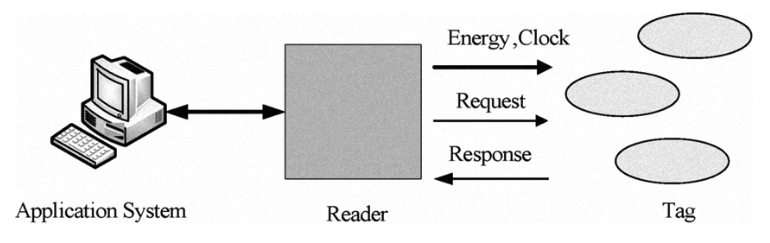
\includegraphics[width=0.5\textwidth]{img/kommunikation.png}}
\caption{Kommunikation zwischen Lesegerät (Reader) und Transponder \cite{b1}}
\label{fig1}
\end{figure}

Das Lesegerät (Reader) induziert über die spulenförmig angeordnete Antenne des Transponders, eine Spannung und Taktfrequenz, welche den Transponder mit dem nötigen Strom versorgt damit eine Kommunikation zwischen Lesegerät und Transponder stattfinden kann. Anschließend sendet das Lesegerät eine Anfrage an den Transponder, woraufhin ihm der Transponder seine Daten die er enthält übermittelt.

Bei den RFID Transpondern wird unterschieden zwischen passiven und aktiven Transpondern.
\begin{itemize}
\item Passive Transponder besitzen keine eigene Spannungsquelle und erreichen dadurch lediglich eine Reichweite von weniger als 4 Metern \cite{b1}.
\item Aktive Transponder hingegen besitzen zusätzlich noch eine eingebaute Spannungsquelle, meist in Form einer Batterie. Dadurch sind Reichweiten von über 100 Metern möglich \cite{b1}.
\end{itemize}
Wie bereits in der Einleitung angemerkt fokussiert sich diese Arbeit ausschließlich auf die passiven Transponder, da diese in im alltäglichen Leben im Gegensatz zu den aktiven Transpondern von größerer Bedeutung sind.

\subsection{NFC Technik}
[WORK IN PROGRESS]

\subsection{Standards}
[WORK IN PROGRESS]

\begin{thebibliography}{00}
\bibitem{b1} Chih-Yung Chen, Chien-Ping Kuo and Fang-Yuan Chien, "An exploration of RFID information security and privacy," 2009 Joint Conferences on Pervasive Computing (JCPC), Tamsui, Taipei, 2009, pp. 65-70, doi: 10.1109/JCPC.2009.5420211.

\bibitem{b2} P. Peng and Y. Zhao, "Anti-cloning and secure RFID mutual authentication protocols," 2011 4th IEEE International Conference on Broadband Network and Multimedia Technology, Shenzhen, 2011, pp. 379-384, doi: 10.1109/ICBNMT.2011.6155961.

\bibitem{b3} Fu K. (2007) Panel: RFID Security and Privacy. In: Dietrich S., Dhamija R. (eds) Financial Cryptography and Data Security. FC 2007. Lecture Notes in Computer Science, vol 4886. Springer, Berlin, Heidelberg
\end{thebibliography}
\end{document}
